Un enseignant d'une classe de CM2 a proposé ce problème à ses élèves.

\medskip
\fbox{
\begin{minipage}{.9\textwidth}
Dans un bocal, un enfant a des billes vertes, des billes rouges et des billes bleues. I/ a 4 fois plus de billes rouges que de billes vertes et il a 3 billes vertes de plus que de billes bleues. En tout il a 51 billes.

Combien a-t-il de billes de chaque couleur ?	
\end{minipage}
}


\begin{flushright}
\scriptsize D'après un problème du Guide pour enseigner la résolution de problèmes au cours moyen, Ministère de l'éducation nationale, 2021	
\end{flushright}


\begin{enumerate}
  \item Voici la réponse proposée par Samira, une élève de la classe de CM2:
\begin{center}
	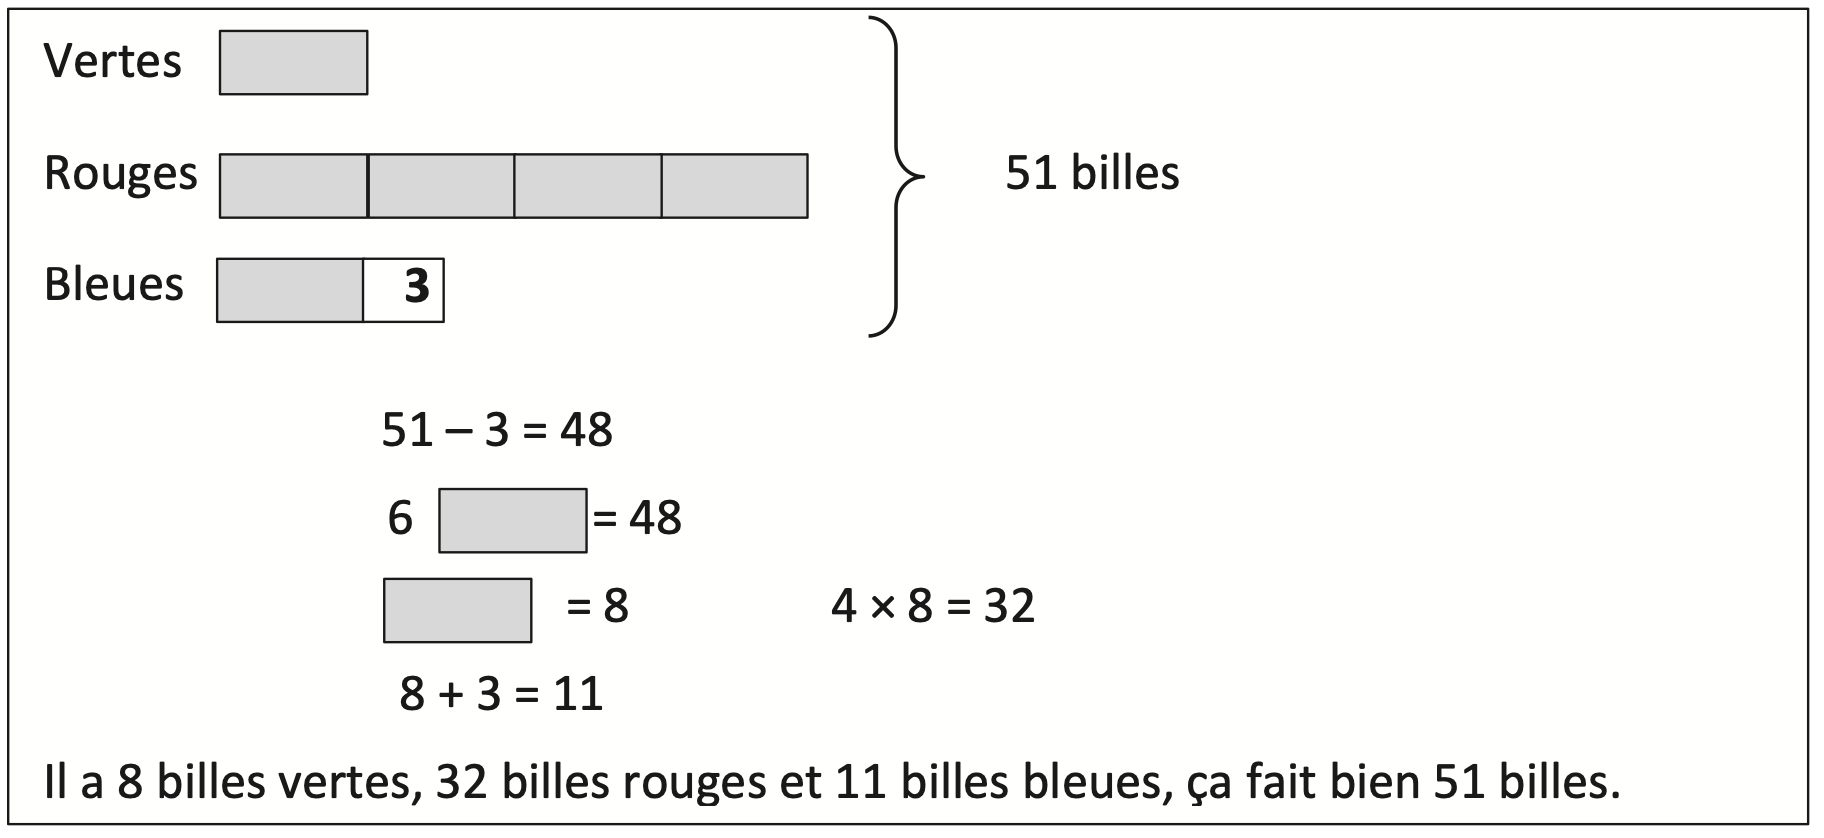
\includegraphics[width=.8\linewidth]{2022-g1-ex3-img1.png}	
\end{center}

Proposer une version corrigée du schéma utilisé par Samira pour résoudre le problème. 

\medskip
\item 
	\begin{enumerate}
		\item En notant $v$ le nombre de billes vertes, déterminer, en fonction de $v$, le nombre de billes rouges et le nombre de billes bleues.
		\item Mettre le problème en équation et la résoudre pour répondre algébriquement à la question posée dans l'énoncé.
	\end{enumerate} 
\end{enumerate}